\centerline{\bf \Huge Power point}

\textbf{Определение.}
Степенью точки $X$ относительно окружности $\omega$ называется величина $\operatorname{Pow}(X, \omega)=d^2-R^2$, где $d-$ расстояние от точки $X$ до центра окружности, а $R$ - радиус окружности.

Если прямая, проходящая через точку $X$, пересекает $\omega$ в точках $A$ и $B$, то степень точки равна $X A \cdot X B$, взятая со знаком «+», если $X$ лежит вне $\omega$, и со знаком «-», если внутри.

\begin{figure}[h]
    \centering
    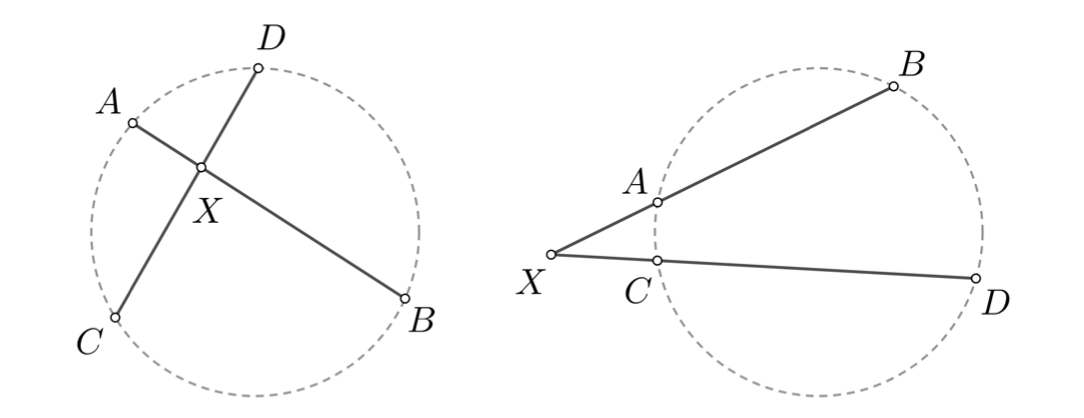
\includegraphics[width=1\linewidth]{Сборы//Зимние сборы 2026//9-10/power_point.png}
    \caption{}
    \label{fig:placeholder}
\end{figure}

\textbf{Утверждение.} Для обеих картинок сверху точки $A, B, C, D$ лежат на одной окружности тогда и только тогда, когда $X A \cdot X B=X C \cdot X D$.

Аналогичные утверждения верны, если секущую заменить на касательную.

\problem{1}
На продолжении хорды $K L$ окружности с центром $O$ взята точка $A$ и из неё проведены касательные $A P$ и $A Q ; M$ - середина $P Q$. Докажите, что $\angle M K O=\angle M L O$.

\problem{2}
В треугольнике $A B C$ отмечены середины $M$ и $N$ отрезков $B C$ и $C M$ соответственно. Описанная окружность треугольника $A B N$ вторично пересекает отрезок $A C$ в точке $S$.
(a) Докажите, что $\angle S M C=\angle M A C$.
(b) Докажите, что $\angle B A M=\angle M S N$.

\problem{3}
Окружность $\omega$ касается сторон угла $B A C$ в точках $B$ и $C$. Прямая $\ell$ пересекает отрезки $A B$ и $A C$ в точках $K$ и $L$ соответственно. Окружность $\omega$ пересекает $\ell$ в точках $P$ и $Q$. Точки $S$ и $T$ выбраны на отрезке $B C$ так, что $K S$ параллельна $A C$ и $L T$ параллельна $A B$. Докажите, что точки $P, Q, S, T$ лежат на одной окружности.

\problem{4}
На высоте $A A_1$ остроугольного треугольника $A B C$ отмечена точка $D$ такая, что $\angle B D C=90^{\circ}$, точка $H$ - ортоцентр треугольника $A B C$. На отрезке $A H$ как на диаметре построена окружность. Докажите, что длина касательной, проведенной к этой окружности из точки $B$, равна длине отрезка $B D$.

\problem{5}
В окружность $\Omega$ вписан шестиугольник $A E C D B F$. Известно, что точка $D$ делит дугу $B C$ пополам, а треугольники $A B C$ и $D E F$ имеют общую вписанную окружность. Прямая $B C$ пересекает отрезки $D F$ и $D E$ в точках $X$ и $Y$, а прямая $E F$ пересекает отрезки $A B$ и $A C$ в точках $Z$ и $T$ соответственно. Докажите, что точки $X, Y, T, Z$ лежат на одной окружности.